\documentclass[10pt,twocolumn,letterpaper]{article}

\usepackage{cvpr}
\usepackage{times}
\usepackage{epsfig}
\usepackage{graphicx}
\usepackage{amsmath}
\usepackage{amssymb}

% Include other packages here, before hyperref.

% If you comment hyperref and then uncomment it, you should delete
% egpaper.aux before re-running latex.  (Or just hit 'q' on the first latex
% run, let it finish, and you should be clear).
\usepackage[breaklinks=true,bookmarks=false]{hyperref}

\cvprfinalcopy % *** Uncomment this line for the final submission

\def\cvprPaperID{****} % *** Enter the CVPR Paper ID here
\def\httilde{\mbox{\tt\raisebox{-.5ex}{\symbol{126}}}}

% Pages are numbered in submission mode, and unnumbered in camera-ready
%\ifcvprfinal\pagestyle{empty}\fi
\setcounter{page}{1}
\begin{document}
	
%%%%%%%%% TITLE\
\title{Term Project Proposal \\
Normal Map Estimation using Model Geometry and Texture \\
Team: Avengers }
\author{Jang Wonjong, Lee Dahun, Jacob Morton\\
	20140337, 20130221, 20172327\\
	Computer Science and Engineering, POSTECH\\
	{\tt\small}}

\maketitle
%\thispagestyle{empty}

%%%%%%%%% BODY TEXT
\section{Introduction}
\subsection{Motivation}
It is an easy task to create a models geometry and texture. There are plenty of 3D modeling software available, like 3D Studio Max, Maya, and blender. It is not too difficult to program or load these into OpenGL as well. The problem of using only 3D geometry and Texture alone can produce flat looking renderings, especially if the geometry is less detailed than the texture. This is typically the case, as texturing can hide simple geometry and flaws. There is more we can do with texture mapping than just wrapping the geometry with an RGB image. We can also add bumb maps, normal maps, displacement maps, and even subsurface scattering to make the rendering more realistic. But these additional mappings are difficult to produce and are often hand-made or produced in multi-step procedures available in some 3D modeling software. Adding a tuned normal to the texture can improve the quality of 3D reconstructed scenes and objects while being illuminated by a light source. We wish for there to be a simple one-step procedure that can take an RGB texture and produce a high-quality normal map that takes into account lighting information.

\begin{figure}[h]
	\begin{center}
		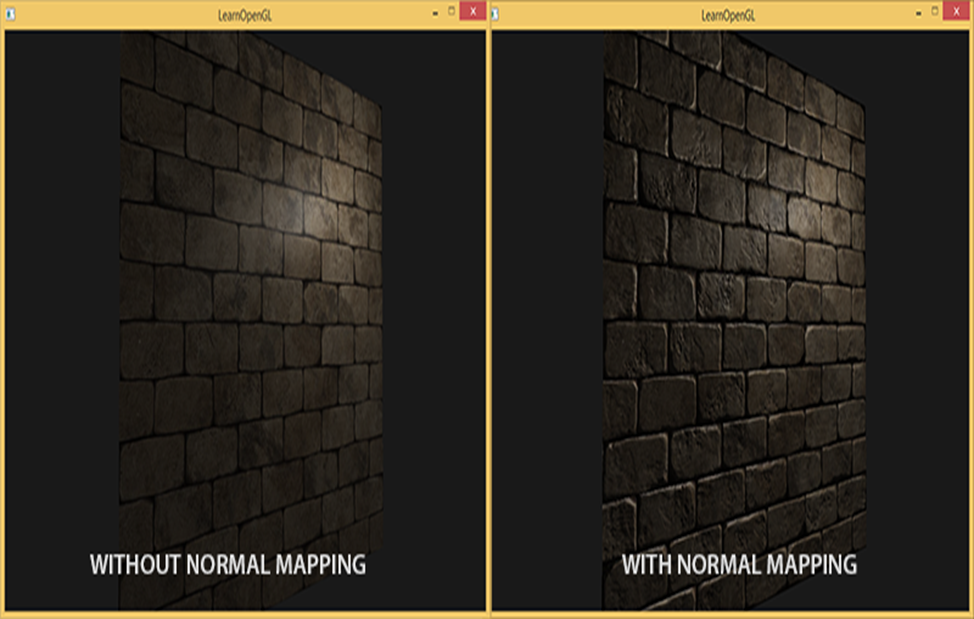
\includegraphics [scale=0.35] {image/wall.png}
		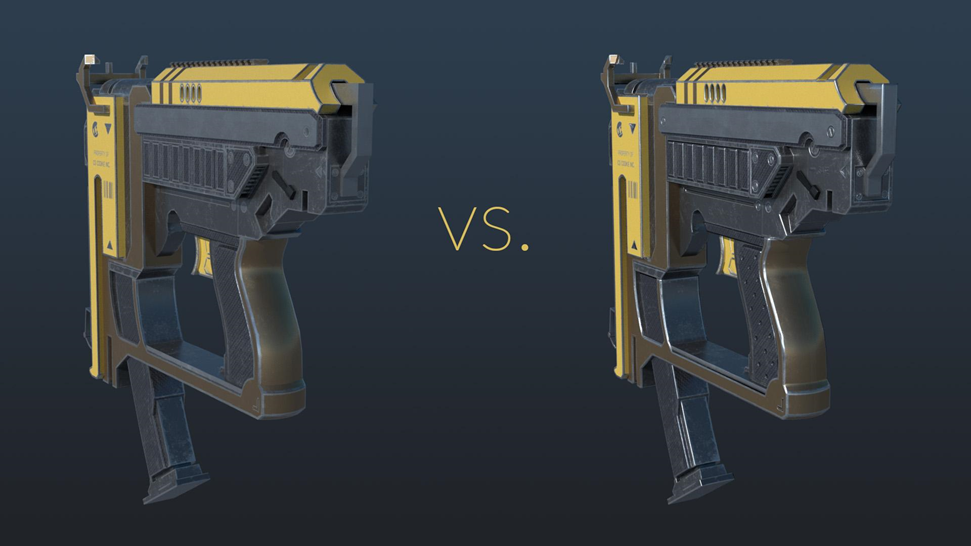
\includegraphics [scale=0.35] {image/gun.png}
	\end{center}
	\caption{Comparison between \textbf{Left:} Geometry + Texture, \textbf{Right:} Geometry + Texture + Normal Map}
	\label{fig:vgg-16}
\end{figure} 

\subsection{Project Description}
We propose a tool for estimating a normal map from a given texture. We will use Spherical Harmonics to estimate the light source direction in the given texture. This lighting direction will be used to compute a per-pixel normal map based on the diffuse surface illumination of the texture. We can then apply this normal map in addition to the model and texture during the texturing process. We will demonstrate this by using a Fragment shader in OpenGL.

\subsection{Background}
This project will require knowledge in Spherical Harmonics, least-squares optimization, normal mapping in OpenGL using fragment shaders.
Using lighting to understand surface topology is very common in 3D Reconstruction and is also something we humans do when viewing an object under lighting. The amount of energy a surface receives is proportional to the angle of a surface to a light source, which is related to the surface normal. We can use Spherical Harmonics (SH) to measure this energy at each pixel on an image and determine the pixel's normal vector. SH often assumes diffuse surface illumination and there may be some error in spectral illumination and self-shadowing. 

\begin{figure}[h]
	\begin{center}
		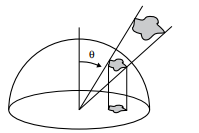
\includegraphics [scale=0.8] {image/energy.png}
	\end{center}
	\caption{light energy illuminated on a surface is proportional to cosine between the surface normal N and the unit vector towards the light source L}
	\label{fig:vgg-16}
\end{figure} 

\section{Development Environment}
\begin{table}[h]
	\begin{tabular}{ll}
		\textbf{Operating System:} &  Windows 10  \\
		\textbf{IDE:} &  MS Visual Studios 2017  \\
		\textbf{Libraries:} &  OpenGL, FreeGlut, GLEW, GLM,\\
		&Ceres Solver, Eigen
	\end{tabular}
\end{table}

\section{Research and Development Plan}
Some time will be needed to understand and implement Spherical Harmonics (SH) for light source estimation. There are plenty of resources available since SH is widely used in the gaming industry for environment illumination. When estimating an environments illumination, SH uses a defined light source to compute the energy of a surface's illumination, which is the inverse of our problem. Also normal map estimation is usually an intermediary step in Shape-From-Shading (SFS), a popular 3D Reconstruction technique. Normal map estimation may also take time to understand. We will use whatever code available to speed up our learning and development time. Our plan is to separate the development tasks so we can work as a team, with equal contribution. The Project will be split up into 3 tasks: SH illumination estimation, Normal map generation from illumination, and rendering.

\subsection{Schedule}
See Table \ref{tab:sched}.
\begin{table}[h]
	\begin{tabular}{l|l}
		\textbf{Date} & Task \\
		\hline
		11/03 - 11/21 & Research, Understand, test examples \\
		11/21 - 12/12 & Implementation \\
		12/12 - 12/21 & Integration and Demo \\
		\hline
	\end{tabular}
	\caption{Schedule}
	\label{tab:sched}
\end{table}

\subsection{Team Member Roles}
See Table \ref{tab:roles}.
\begin{table}[h]
	\begin{tabular}{l|l}
		\textbf{Name} & Roles \\
		\hline
		WonJong & SH and Light source Estimation \\
		Dahun & Rendering Model, Texture, and Normal Map \\
		Jake & SH and Normal Map generation \\
		\hline
	\end{tabular}
	\caption{Team Member Roles}
	\label{tab:roles}
\end{table}

\begin{thebibliography}{1}
	\bibitem{green} 
	R. Green.
	\textit{Spherical Harmonic Lighting: The Gritty Details}. 
	GDC 2003.
	
	\bibitem{dicky} 
	Rich Forster.
	\textit{Spherical Harmonics for Beginners}. 
	https://dickyjim.wordpress.com/2013/09/04/spherical-harmonics-for-beginners/
	
	
	\bibitem{igor} 
	Igor Goldvekht. 
	\textit{Shape-From-Shading}. 
	https://github.com/IgorGee/Shapes-From-Shading
\end{thebibliography}

\end{document}
